\chapter{Aplicación}
\label{chap:aplicacion}
En esta sección se presenta la aplicación del framework para evaluar mantenibilidad
sobre un producto de software real. Se parte definiendo las tareas correspondientes
al proceso de evaluación, para luego continuar con la ejecución de la evaluación
utilizando el modelo presentado en la propuesta.

\section{Requerimientos de la evaluación}

\subsection{Propósito de la evaluación}

Se desea evaluar el producto de software SAE de la empresa MOSAQ con el fin de
elaborar un plan de calidad que permita cerrar brechas en torno a temas de
mantenibilidad de su producto. A través de esta evaluación se acreditará que la
empresa utilizó un conjunto de buenas prácticas para construir el software y que
éste puede ser mantenido y modificado por terceros en el caso que fuese necesario.

\subsection{Requerimientos de calidad del producto de software}

El principal requerimiento del producto es la mantenibilidad. Se desea evaluar
la continuidad de desarrollo del producto para certificar su correctitud
en caso de que terceros deban tomar el desarrollo.

\subsection{Partes del producto sometidas a evaluación}

Se sometieron a evaluación dos módulos del producto de software. Estos son SAE Framework
Servidor y SAE Framework Cliente. La evaluación difiere en algunos aspectos para cada módulo
puesto que tienen diferencias en su arquitectura.

\subsection{Rigor de la evaluación}

Se decidió que la mayor cantidad de esfuerzo y rigor debe estar enfocado en estudiar y
analizar la mantenibilidad del producto.

Se estudiaron a fondo métricas relacionadas con la mantenibilidad del producto y se
utilizaron criterios que permiten asegurar prácticas profesionales en la construcción
del producto de software.

También se realizaron descripciones cualitativas acerca de la portabilidad del producto.
Esta característica junto con la mantenibilidad, es importante para los clientes de MOSAQ
ya que ambas influyen en los procesos que se deben llevar a cabo en el caso de que se tuviese
que trabajar con terceros en un futuro.
\label{chap:validation}

\section{Diseño de la evaluación}
Para llevar a cabo las mediciones, MOSAQ hizo entrega de las fuentes principales de su software,
los cuales bajo un acuerdo de confidencialidad, fueron analizados por parte del equipo Toeska.

\subsection{Para SAEFramework Servidor}
Las mediciones para este módulo se realizaron con las siguientes herramientas:

\begin{itemize}
\item NDepend v5.0.0.8085\footnote{http://www.ndepend.com}
\item Visual Studio 2013 Code Metrics\footnote{http://msdn.microsoft.com/en-us/library/bb385914.aspx}
\item Visual Studio 2012 Code Clone Analysis\footnote{http://msdn.microsoft.com/en-us/library/hh205279.aspx}
\end{itemize}

\subsection{Para SAEFramework Cliente}

\begin{itemize}
\item SonarQube\footnote{http://www.sonarqube.org/}
\item JsHint v2.1.11\footnote{http://www.jshint.com/}
\item WebStorm v7 Inspection tools\footnote{http://www.jetbrains.com/webstorm/}


La configuración elegida para JsHint es la siguiente:
\begin{verbatim}
{
    "globals": {
        "console": false,
        "jQuery": false,
        "_": false
    },
    "maxparams": 5,
    "maxdepth": 5,
    "maxstatements": 25,
    "maxcomplexity": 10,
    "es5": true,
    "browser": true,
    "boss": false,
    "curly": false,
    "debug": false,
    "devel": false,
    "eqeqeq": true,
    "evil": true,
    "forin": false,
    "immed": true,
    "laxbreak": false,
    "newcap": true,
    "noarg": true,
    "noempty": false,
    "nonew": false,
    "nomen": false,
    "onevar": true,
    "plusplus": false,
    "regexp": false,
    "undef": true,
    "sub": true,
    "strict": false,
    "white": true,
    "unused": true
}
\end{verbatim}

En esta configuración podemos ver los parámetros \textit{maxparams}, \textit{maxdepth} 
y \textit{maxcomplexity} los cuales nos permiten definir los límites para el número de parámetros,
profundidad y complejidad ciclomática respectivamente. Estos parámetros fueron seleccionados de manera
informada de acuerdo a buenas prácticas investigadas previamente y acordes a un software con las
características de SAE Framework.
\end{itemize}

% PLAN DE ACTIVIDADES DE EVALUACION %
\subsection{Plan de actividades de evaluación}

A través de reuniones con MOSAQ, se acordaron los siguientes puntos dentro del plan de trabajo en lo
que respecta a planificación y evaluación de calidad.
\begin{itemize}
\item El equipo Toeska realizará las mediciones pertinentes sobre el código fuente y sobre algunas
prácticas de desarrollo del equipo de MOSAQ. Con estas mediciones se evaluarán los requerimientos de
calidad establecidos en el modelo utilizado para evaluar.

\item El equipo Toeska entregará los resultados de la primera evaluación, los puntos donde se encontraron
brechas que deben ser consideradas, y guías para realizar los ajustes necesarios para que el producto
obtenga mejores resultados durante la próxima evaluación.

\item Finalmente se realizará otra evaluación utilizando los mismo criterios utilizados
para la primera evaluación, en la cual se espera haber cerrado las brechas encontradas anteriormente
y así certificar que el producto cumple con las características escogidas del modelo.
\end{itemize}

\section{Resultados de la primera evaluación SAEFramework Servidor}
\subsection{Realización de mediciones de mantenibilidad}

\subsubsection{Cohesión Relacional}

Los resultados para esta métrica se pueden observar en el cuadro número~\ref{table:CR}.

\begin{table}
  \small
\centering
    \begin{tabular}{|l|l|l|}
    \hline
       \bf{Assemblies}       & \bf{Cohesión Relacional} & \bf{Nombre}           \\ \hline
       SaeFramework2013 & 1.4                   & SaeFramework2013 \\ \hline
    \end{tabular}
    \caption{Cohesión relacional}
    \label{table:CR}
\end{table}

\subsubsection{LCOM}

Los resultados de esta métrica se pueden ver en el cuadro~\ref{table:LOCM}.

\begin{table}
  \small
\centering
    \begin{tabular}{|l|l|}
    \hline
    \bf{Nombre}                                                         & \bf{LCOM}    \\ \hline
       Mosaq.SaeFramework.v2013.Vistas.ListadoAuditoriaTicket      &    0.97 \\ \hline
       Mosaq.SaeFramework.v2013.Negocio.CreacionOSTicket           &    0.82 \\ \hline
       Mosaq.SaeFramework.v2013.Negocio.EdicionTicket              &    0.78 \\ \hline
       Mosaq.SaeFramework.v2013.Datos.Conector                     &    0.68 \\ \hline
       Mosaq.SaeFramework.v2013.Negocio.ManutencionCentroCosto     &    0.5  \\ \hline
       Mosaq.SaeFramework.v2013.Negocio.ManutencionCoberturaSitios &    0.42 \\ \hline
       Mosaq.SaeFramework.v2013.Negocio.ManutencionZonas           &    0.42 \\ \hline
    \end{tabular}
	\caption{Principales tipos y su LCOM}
    \label{table:LOCM}
\end{table}

\subsubsection{LCOM HS}
Los datos del análisis para LCOM HS se pueden observar en el cuadro~\ref{table:LOCMHS}
\begin{table}
  \small
\centering
    \begin{tabular}{|l|l|}
    \hline
    \bf{Nombre}                                                    & \bf{LCOMHS} \\ \hline
       Mosaq.SaeFramework.v2013.Vistas.ListadoAuditoriaTicket      &    1        \\ \hline
       Mosaq.SaeFramework.v2013.Negocio.CreacionOSTicket           &    0.9      \\ \hline
       Mosaq.SaeFramework.v2013.Negocio.EdicionTicket              &    0.88     \\ \hline
       Mosaq.SaeFramework.v2013.Datos.Conector                     &    0.71     \\ \hline
       Mosaq.SaeFramework.v2013.Negocio.ManutencionCentroCosto     &    0.67     \\ \hline
       Mosaq.SaeFramework.v2013.Negocio.ManutencionCoberturaSitios &    0.56     \\ \hline
       Mosaq.SaeFramework.v2013.Negocio.ManutencionZonas           &    0.56     \\ \hline
       Mosaq.SaeFramework.v2013.Utilidades.StringEnum              &    0.5      \\ \hline
    \end{tabular}
    \caption{Principales tipos y su LCOM HS}
    \label{table:LOCMHS}
\end{table}


\subsubsection{Acoplamiento eferente}
Las mediciones para los $10$ tipos con mayor valor de acoplamiento eferente se pueden observar en el cuadro~\ref{table:EC}.
\begin{table}
    \small
\centering
    \begin{tabular}{|l|l|}
    \hline
    \bf{Nombre}                                                    & \bf{Tipos que utiliza} \\ \hline
       Mosaq.SaeFramework.v2013.Vistas.ConsultaVistas              &    89                  \\ \hline
       Mosaq.SaeFramework.v2013.Negocio.TicketAcciones             &    34                  \\ \hline
       Mosaq.SaeFramework.v2013.Negocio.ReglasNegocio              &    28                  \\ \hline
       Mosaq.SaeFramework.v2013.Negocio.CreacionOSTicket           &    22                  \\ \hline
       Mosaq.SaeFramework.Utilidades.TypeMap                       &    26                  \\ \hline
       Mosaq.SaeFramework.v2013.Datos.Conector                     &    24                  \\ \hline
       Mosaq.SaeFramework.v2013.Utilidades.Utilidades              &    21                  \\ \hline
       Mosaq.SaeFramework.v2013.Standard.CmdbComponentes           &    20                  \\ \hline
       Mosaq.SaeFramework.v2013.Standard.GruposResolutoresEmpresas &    19                  \\ \hline
       Mosaq.SaeFramework.v2013.Standard.ZonasEmpresas             &    19                  \\ \hline
    \end{tabular}
    \caption{Top 10 de tipos y su acoplamiento eferente}
    \label{table:EC}
\end{table}


\subsubsection{Acoplamiento aferente}

Las mediciones para los $10$ tipos con mayor valor de acoplamiento aferente se pueden observar en el cuadro~\ref{table:AC}.

\begin{table}
    \footnotesize
\centering
    \begin{tabular}{|l|l|}
    \hline
    \bf{Nombre del método}                                                                               & \bf{Métodos que lo utilizan} \\ \hline
       Mosaq.SaeFramework.v2013.Datos.Conector.fabricar()                                                  &    425                         \\ \hline
       Mosaq.SaeFramework.v2013.Datos.IConector.ejecutarProcedimiento                    &    237                         \\ \hline
       Mosaq.SaeFramework.v2013.Datos.IConector.extraerProcedimientoI    &    161                         \\ \hline
       Mosaq.SaeFramework.v2013.Datos.IConector.ejecutarProcedimientoInt                    &    130                         \\ \hline
       Mosaq.SaeFramework.v2013.Datos.IConector.retornaListaI                               &    14                          \\ \hline
       Mosaq.SaeFramework.v2013.Datos.IConector.IniciaTransaccion()                                        &    12                          \\ \hline
       Mosaq.SaeFramework.v2013.Datos.IConector.EjecutaTransaccion()                                       &    12                          \\ \hline
       Mosaq.SaeFramework.v2013.Datos.IConector.CancelaTransaccion()                                       &    12                          \\ \hline
    \end{tabular}
    \caption{Top 10 de métodos y su acoplamiento aferente}
    \label{table:AC}
\end{table}


\subsubsection{Código muerto}
Total: \textbf{581 métodos}.

\subsubsection{Instabilidad}

Para el cálculo de esta medida se utilizó el promedio del Top 10 de tipos con
mayor acoplamiento eferente y el promedio del Top 10 de los tipos con mayor
acoplamiento aferente. Estos valores se pueden obtener utilizando los datos
de las tablas anteriores. A continuación se presenta el resultado.

$$I = 30.2 / (30.2 + 102.3)$$
$$I = 0.23$$
\subsubsection{Complejidad ciclomática}

En el cuadro~\ref{table:CC} se pueden observar los 10 métodos con mayor complejidad ciclomática.

\begin{table}
    \small
\centering
    \begin{tabular}{|l|l|}
    \hline
    \bf{Nombre}                                                                          & \bf{Complejidad ciclomática} \\ \hline
       Vistas.ConsultaVistas.Lista                              &    77                          \\ \hline
       Negocio.TicketAcciones.Transferir                        &    10                          \\ \hline
       Negocio.TicketAcciones.ReabrirTicket                     &    8                           \\ \hline
       Negocio.TicketAcciones.Recatalogar                       &    5                           \\ \hline
       Negocio.TicketAcciones.ProgramarFechaAtencion            &    4                           \\ \hline
       Negocio.CreacionOSTicket.grabarYcalcularFechasTickets &    4                           \\ \hline
       Utilidades.Validadores.digitoVerificador                       &    5                           \\ \hline
       Utilidades.StringEnum.Parse                              &    5                           \\ \hline
       Utilidades.Utilidades.IEnumerableToDataTable        &    5                           \\ \hline
       Datos.Conector.ejecutarProcedimientoCadenaAnidada     &    4                           \\ \hline
    \end{tabular}
    \caption{Top 10 de métodos y su complejidad ciclomática}
    \label{table:CC}
\end{table}


\subsubsection{Índice de mantenibilidad}
En el cuadro~\ref{table:MI} se muestra el valor del índice de mantenibilidad para el código de software.
\begin{table}
  \small
\centering
    \begin{tabular}{|l|l|}
    \hline
    \bf{Nombre}      & \bf{Índice de mantenibilidad} \\ \hline
    SaeFramework2013 & 93                              \\ \hline
    \end{tabular}
    \caption{Índice de mantenibilidad}
    \label{table:MI}
\end{table}

\subsubsection{Código duplicado}

En el cuadro~\ref{table:clones} se pueden observar los clones de código
encontrados en el software. En la primera columna se presenta el grupo y la
intensidad de la duplicación encontrada, mientras que en la segunda columna el
nombre de los archivos y las líneas donde se encontró el código duplicado.

\begin{table}
    \small
\centering

  \begin{tabular}{ | l | l | }
  
  \hline
    \bf{Grupo de Clones} & \bf{Nombre} \\ \hline
    Match Fuerte (1 archivo) & Negocio\textbackslash TicketAcciones.cs líneas 75-94 \\ \hline
     & Negocio\textbackslash TicketAcciones.cs líneas 360-380 \\ \hline
    Match Medio (2 archivos) & Negocio\textbackslash ManutencionCoberturaSitios.cs líneas 69-94 \\ \hline
     & Negocio\textbackslash ManutencionZonas.cs líneas 69-94 \\ \hline
    Match Débil (1 archivo) & Negocio\textbackslash TicketAcciones.cs líneas 119-143 \\ \hline
     & Negocio\textbackslash TicketAcciones.cs líneas 304-329 \\ \hline
     & Negocio\textbackslash TicketAcciones.cs líneas 207-231 \\ \hline
     & Negocio\textbackslash TicketAcciones.cs líneas 43-65 \\ \hline
    Match Débil (2 archivos) & Negocio\textbackslash ManutencionCoberturaSitios.cs líneas 103-127 \\ \hline
     & Negocio\textbackslash ManutencionZonas.cs líneas 104-128 \\ \hline
  \end{tabular}
  \caption{Clones de código}
  \label{table:clones}
\end{table}

\subsection{Realización de mediciones de portabilidad}

\subsubsection{Observaciones}
\begin{itemize}
\item Se debe obtener documentación necesaria por parte de MOSAQ para analizar
las prácticas habituales con respecto a temas de instalabilidad y así proponer recomendaciones.
\end{itemize}

%---------------------------------------RESULTADOS PARA SAE CLIENTE -----------------------------------------%
\section{Resultados de la primera evaluación SAEFramework Cliente}

Para el estudio de este módulo se evaluaron los siguientes directorios y archivos:
\begin{itemize}
\item Js/app.js
\item Js/BasePrincipal.js
\item Js/controllers
\item Js/app/connection/wcf.js
\item Js/app/services/services.js
\end{itemize}

\subsection{Realización de mediciones para mantenibilidad}
\subsubsection{Complejidad Ciclomática}

En el cuadro~\ref{table:JSCC} se pueden observar los archivos y directorios
seleccionados para la evaluación, así como su respectiva complejidad por método.
\begin{table}
  \small
\centering
    \begin{tabular}{|l|l|}
    \hline
    \textbf{Archivo/Directorio}            & \textbf{Complejidad por método} \\ \hline
    app.js                        & 4.1                    \\ \hline
    BasePrincipal.js              & 3.0                    \\ \hline
    app/controllers/debug         & 1.2                    \\ \hline
    app/controllers/admin         & 1.7                    \\ \hline
    app/controllers/laboratorio   & 1.0                    \\ \hline
    app/controllers/main          & 1.9                    \\ \hline
    app/controllers/ordenservicio & 1.7                    \\ \hline
    app/controllers/tickets       & 2.2                    \\ \hline
    app/connection/wcf.js         & 4.1                    \\ \hline
    app/services/services.js      & 1.8                    \\ \hline
    \end{tabular}
    \caption{Elementos elegidos y su complejidad por método}
    \label{table:JSCC}
\end{table}

\subsubsection{Profundidad}
En el cuadro~\ref{table:depth} se pueden observar los archivos y directorios
seleccionados para la evaluación y su análisis respectivo de profundidad. Se
debe recordar que se eligió utilizar un valor de 5 como mínimo para que el
elemento sea considerado como crítico.
\begin{table}
  \small
\centering
    \begin{tabular}{|l|l|}
    \hline
    \textbf{Archivo/Directorio}            & \textbf{Profundidad}                 \\ \hline
    app.js                        & Sin profundidad mayor que 5 \\ \hline
    BasePrincipal.js              & Sin profundidad mayor que 5 \\ \hline
    app/controllers/debug         & Sin profundidad mayor que 5 \\ \hline
    app/controllers/admin         & Sin profundidad mayor que 5 \\ \hline
    app/controllers/laboratorio   & Sin profundidad mayor que 5 \\ \hline
    app/controllers/main          & Sin profundidad mayor que 5 \\ \hline
    app/controllers/ordenservicio & Sin profundidad mayor que 5 \\ \hline
    app/controllers/tickets       & Sin profundidad mayor que 5 \\ \hline
    app/connection/wcf.js         & Sin profundidad mayor que 5 \\ \hline
    app/services/services.js      & Sin profundidad mayor que 5 \\ \hline
    \end{tabular}
    \caption{Elementos elegidos y el match para profundidad seleccionado}
    \label{table:depth}
\end{table}
\subsubsection{Número de parámetros}

En el cuadro~\ref{table:PN} se pueden observar los archivos y directorios
seleccionados para la evaluación y su análisis respectivo del número de
parámetros en sus funciones. Para esta métrica se decidió utilizar un mínimo
de 5 parámetros para considerar un elemento como peligroso.
\begin{table}
  \small
\centering
    \begin{tabular}{|l|l|}
    \hline
    Archivo/Directorio            & Número de parámetros \\ \hline
    app.js                        & No sobrepasa             \\ \hline
    BasePrincipal.js              & No sobrepasa             \\ \hline
    app/controllers/debug         & No sobrepasa             \\ \hline
    app/controllers/admin         & No sobrepasa             \\ \hline
    app/controllers/laboratorio   & No sobrepasa             \\ \hline
    app/controllers/main          & No sobrepasa             \\ \hline
    app/controllers/ordenservicio & No sobrepasa             \\ \hline
    app/controllers/tickets       & No sobrepasa             \\ \hline
    app/connection/wcf.js         & No sobrepasa             \\ \hline
    app/services/services.js      & No sobrepasa             \\ \hline
    \end{tabular}
    \caption{Elementos elegidos y el match para número de parámetros seleccionado}
    \label{table:PN}
\end{table}
\subsubsection{Código duplicado}

No se han encontrado registros de código duplicado relevante. El análisis
sólo entregó duplicación con respecto a la versión minificada del software,
lo cual no corresponde a duplicación que afecte la mantenibilidad.

\section{Conclusiones SAEFramework Servidor}

\subsection{Mantenibilidad}

El primer valor analizado es el de Cohesión relacional. El valor para este
análisis es de 1.4. Este resultado se encuentra dentro del rango considerado
como correcto para una aplicación. Valores más altos podrían indicar
sobre-acoplamiento ya que la cohesión relacional nos entrega un promedio
de relaciones internas por tipo dentro de un paquete. Un paquete debe tener
sus clases fuertemente relacionadas y estas no deberían estar relacionadas de manera
considerable con clases externas.

Las siguientes métricas corresponden a LCOM y LCOM HS. Para estas medidas existen rangos definidos que
son considerados como correctos para un conjunto de tipos.

Con respecto a LCOM, se deben analizar los tipos que tengan un valor
mayor a 0.8. En este caso existen 2 tipos que sobrepasan ese valor. Estos tipos son:
\begin{itemize}
\item CreacionOSTicket (Clase)
\item ListadoAuditoriaTicket (Clase)	
\end{itemize}

Se han analizado estas clases y se concluyó que no es necesario realizar
cambios sobre ellas ya que sólo están compuestas por \textit{getters}
y \textit{setters}. Las clases de este estilo no son correctamente evaluadas
por esta métrica ya que no tienen un comportamiento definido por relaciones
entre sus métodos.

Para los valores de LCOM HS se recomienda analizar los tipos cuyos resultados
sean estrictamente mayores que 1. En las mediciones no se encontraron tipo
que sobrepasen este umbral. Solo la clase \textbf{ListadoAuditoriaTicket}
arrojó un valor igual a 1, sin embargo por las razones explicadas en el análisis
de LCOM, esta clase no está mal implementada de acuerdo a esta métrica.

El valor de \textbf{acoplamiento eferente} podría revelar tipos que tienen
muchas responsabilidades. Mientras mayor sea este valor, más entrelazado está
el tipo con otras implementaciones. Si bien los valores obtenidos no son altos,
se recomienda analizar los primeros tipos y verificar si pueden ser más modularizados.

Para la métrica de \textbf{acoplamiento aferente} se pueden observar el top 10
de los tipos con mayores llamadas dentro del sistema. Estos valores no indican
problemas de diseño y sirven para estudiar cuales son los tipos más utilizados.
Esta información se entrega con el fín de obtener un estudio más detallado
acerca del software.

Con respecto al \textbf{código muerto}, se entrega una planilla con los métodos
para los cuales se encontraron 0 llamadas (no incluida en este trabajo).
Se recomienda analizar estos métodos y verificar si realmente son
necesarios en el sistema o de lo contrario eliminarlos ya que pueden degradar
la analizabilidad del software.

El valor de \textbf{instabilidad} es de 0.23. Este valor puede variar entre
0 y 1, donde 0 indica un paquete completamente estable y 1 un paquete
completamente inestable. El valor obtenido en este caso es bastante aceptable
e indica que el software se encuentra en un estado estable y tiene una buena
modificabilidad. Cabe mencionar que este valor se obtiene analizando las
métricas de acoplamiento descritas anteriormente, de esta manera este valor
esta relacionado con el nivel de acoplamiento en el sistema.

Para la \textbf{complejidad ciclomática} se muestra una tabla con
el top 10 de los métodos con la mayor complejidad. El estándar indica
que un método con una complejidad ciclomática mayor a 30 puede
ser demasiado complejo y se debe estudiar la posibilidad de dividirlo en
métodos más pequeños a menos que corresponda a código generado automáticamente.
En este caso el análisis arrojó sólo un método con un valor superior a 30,
el cual es \textbf{Listar()} dentro de \textbf{Vistas.ConsultaVistas}.
Se analizó este método y se puede observar de que contiene un \textit{switch}
con un gran número de \textit{cases}. Este \textit{switch} es el que genera
un aumento en la complejidad ciclomática. Por lo tanto se recomienda estudiar
este método y buscar alguna manera de refactorizar para obtener un código
más mantenible. Algunas opciones para este tipo de refactorización
se basan en utilizar diccionarios, mapas o simplemente separar las enumeraciones
en sus propias clases.

El valor obtenido para el \textbf{índice de mantenibilidad} es de 93. Este
valor puede estar entre 0 y 100 y mientras más alto indica una mejor
mantenibilidad. En este caso el valor sugiere que el software es altamente
mantenible bajo los estándares de esta métrica.

Finalmente, el análisis de código duplicado entrega una tabla en la cual se
pueden observar archivos que contienen posibles fuentes de código duplicado.
Si bien este análisis muestra que el código duplicado es mínimo, se recomienda
estudiar estos archivos y ver si se puede refactorizar código para así disminuir
aún más la cantidad de duplicación.
%-----------------------------CONCLUSIONES CLIENTE-----------------------------------------------------%

\section{Conclusiones SAEFramework Cliente}

\subsection{Mantenibilidad}

Para este módulo no se encontraron deficiencias relevantes con respecto a la
mantenibilidad del código.

Para realizar el análisis se debe tener en cuenta que la arquitectura para
esta parte del framework difiere profundamente con la arquitectura servidor.
Esto es debido al uso de herramientas nuevas que utilizan javascript a través
de patrones de diseño que clásicamente no se aplicaban en ingeniería de \textit{front-end}.

Para la complejidad ciclomática se debe estudiar la complejidad por
método y no por archivo, puesto que en esta arquitectura un archivo no
necesariamente representa a una clase y usualmente define una serie de funciones
asíncronas definidas para su framework. Es por esto que la complejidad
ciclomática de un archivo puede resultar alta, sin embargo por método es baja.
Luego de estudiar los archivos y directorio elegidos, no se encontraron métodos
con complejidad alta por lo cual esta parte del código tiene buena mantenibilidad
con respecto a sus complejidad.

Al encontrar funciones con un valor de profundidad muy alto, se generan
problemas de analizabilidad y por ende de mantenibilidad. Para este caso,
como es un framework de mediana magnitud, se decidió utilizar un valor de 5
anidaciones para no ser demasiado restrictivo, ni demasiado permisivo.
Al realizar el análisis no se encontró ningún elemento que sobrepase este
umbral, por lo cual esta característica no está afectando la analizabilidad del
sistema.

EL número de parámetros que un método recibe también es una métrica que se debe
tener en cuenta para estudiar la analizabilidad de un sistema. Mientras más
parámetros recibe una función, más compleja se vuelve su analizabilidad y
mantenibilidad. En este caso utilizando los mismo argumentos que en la métrica
anterior, se escogió un número de 5 parámetros como mínimo para considerar a
una función como crítica. Luego de realizar el análisis, no se encontraron
funciones que sobrepasen este umbral, por lo cual esta es otra característica
bien implementada en el sistema y que mejora su mantenibilidad.

Finalmente como se mencionó en la sección anterior, el software que se utilizó
para realizar las mediciones de duplicación, sólo entregó duplicaciones de
varios archivos con respecto a la versión minificada del framework, por ende
no son consideradas.

\section{Recomendaciones}

Para ambos módulos se recomienda el uso de alguna herramienta de análisis
de código estático. Estas herramientas permiten estudiar algunas de las métricas
presentadas en este informe así como buenas prácticas correspondientes al
lenguaje de la aplicación.
Los valores adecuados para cada métrica se pueden encontrar en la
sección de especificación del modelo de calidad.

Para el código de SAE Servidor se pueden utilizar las métricas de código
ofrecidas por Visual Studio. A través de estas métricas se puede analizar el
índice de mantenibilidad con el fin de que no se escape de los márgenes
apropiados. Este análisis debe ser complementado con alguna otra herramienta
de análisis estático. Se estudiaron 2 herramientas las cuales tienen ciertas
ventajas y desventajas.

La primera herramienta es \textbf{NDepend}, la cual se utilizó para obtener la mayoría
de las métricas que se presentaron en la sección de análisis de SAE Servidor.
Esta herramienta es altamente profesional, se integra de manera perfecta con
Visual Studio y entrega reportes muy detallados. Este software es propietario
y tiene un costo asociado.

Por otro lado se analizó la herramienta \textbf{SonarQube}, la cual se utilizó para
obtener la mayoría de medidas para SAE Cliente. Este software también tiene
una extensión para .NET lo cual permitió realizar pruebas sobre el código
fuente del lado servidor.
SonarQube presenta buenos resultados, los cuales pueden ser útiles para
perpetuar la mantenibilidad del código. Además, esta herramienta es de código
abierto lo cual la ubica como la mejor opción puesto que no se desea hacer un
análisis demasiado exhaustivo sino más bien encontrar puntos críticos dentro
del producto que puedan afectar su mantenibilidad. El uso de Sonarqube también
se recomienda para analizar el código del lado cliente.

\section{Evaluación final para SAEFramework Servidor}
La evaluación final se realizó utilizando la versión más reciente del producto
SAE Framework Servidor. Para esta evaluación se incluyen además observaciones
con respecto a otras características que no se encuentran en la primera evaluación y
que corresponden a Instalabilidad y la subcaracterística capacidad de pruebas.
Esta última comenzó a ser implementada durante el transcurso de la evaluación
por lo que inicialmente no se contaba con pruebas de software.
A continuación se presenta una síntesis de las métricas más relevantes para
este punto de la evaluación.

\subsection{Mediciones de mantenibilidad}

\subsubsection{Cohesión relacional}
Se obtuvo un valor similar al de la primera evaluación.
\subsubsection{LCOM}
Se obtuvieron valores similares a los de la primera evaluación para el Top 10 de métodos
con mayor valor para esta métrica.
\subsubsection{LCOM HS}
Se obtuvieron valores similares a los de la primera evaluación para el Top 10 de métodos
con mayor valor para esta métrica.
\subsubsection{Acoplamiento Eferente}
Se obtuvieron valores similares a los de la evaluación anterior, sin embargo esta vez no aparece en primer lugar
el método ConsultaVistas(), el cual sobrepasaba el umbral de acoplamiento recomendable.
\subsubsection{Acoplamiento Aferente}
Se obtuvieron valores similares a los de la evaluación anterior.
\subsubsection{Instabilidad}
Nuevo valor obtenido: 0.18.
Este valor descendió debido a que el acoplamiento eferente ya no aumenta
demasiado su valor, gracias a la refactorización del método con mayor valor obtenido en la primera evaluación.
Cabe recordar que mientras más bajo sea este valor, más mantenible es el producto de software.
\subsubsection{Complejidad Ciclomática}
Al igual que en acoplamiento eferente, el método ConsultarVista() ya no lidera el top 10 de métodos
con mayor complejidad. Este método agregaba un valor de complejidad
ciclomática de 77 en la primera evaluación, el cual ya no aparece en el ranking.
De esta manera el método con mayor complejidad tiene un valor de 10 y
corresponde al segundo en la lista de la primera evaluación. El resto de la lista
es similar.
\subsubsection{índice de Mantenibilidad}
El índice de mantenibilidad entregado por la herramienta \textit{Code metrics} de Visual Studio 2012
aún entrega un excelente valor de 93.
\subsubsection{Código Duplicado}
El análisis de \textit{Code Clones} provisto por Visual Studio 2012 entregó matches para los
mismos archivos descritos en la primera evaluación.
\subsection{Capacidad de Pruebas}
\label{cap}

La capacidad para realizar pruebas en el software es fundamental para un producto mantenible y es por eso
que MOSAQ ha decidido implementar esta propuesta.

Inicialmente se tenía un 0\% de cobertura de pruebas y durante el desarrollo de
la evaluación, el equipo Toeska entregó un plan para comenzar a implementar
módulos de pruebas y un ambiente de testing para el equipo de desarrollo.

Se clasificaron diferentes servicios y sus respectivas pruebas de acuerdo a su criticidad.
En el cuadro~\ref{table:CBPC} se puede observar el total de pruebas para cada
categoría, mientras que en el cuadro~\ref{table:CBC} se presenta el cumplimiento
para estas mismas de acuerdo a los rangos recomendados por el equipo Toeska.

Con esta información podemos concluir que esta característica se cumple correctamente.
\begin{table}
  \small
\centering
    \begin{tabular}{lll}
    ~               & Total  & \%        \\
     		Críticas:    &  		12  &  		8.51   \\
     		Importantes: &  		28  &  		19.86  \\
     		Deseables:   &  		101 &  		71.63  \\
     		Todas        &  		141 &  		100.00 \\ \hline
    \end{tabular}
     \caption{Cobertura de pruebas - porcentaje por criticidad}
    \label{table:CBPC}
\end{table}

\begin{table}
  \small
\centering
    \begin{tabular}{llllll}
    ~               &  		Total &  		Faltan &  		\% Real &  		\% Meta & ¿Cumple? \\
     		Críticas:    &  		12    & 0         &  		100.00 &  		100.00 &  		SI    \\
     		Importantes: &  		28    & 0         &  		100.00 &  		80.00  &  		SI    \\
     		Deseables:   &  		101   & 0         &  		100.00 &  		40.00  &  		SI    \\
     		Todas        &  		141   & ~         & ~         & ~         & ~        \\ \hline
    \end{tabular}
         \caption{Cobertura de pruebas - Cumplimiento}
    \label{table:CBC}
\end{table}

\subsection{Portabilidad (Instalabilidad)}
\label{ins}
Para esta etapa de la evaluación se evaluó también la Instalabilidad del software.
Esta característica toma fuerte relevancia en el caso de que terceros deban mantener el software a futuro.

Para realizar este análisis se estudió un documento provisto por MOSAQ, el cual
muestra la información relevante de los procesos involucrados en la instalación del software.
En este documento se especifica entre otras cosas:

\begin{itemize}
\item Los pre-requisitos de Hardware y Software que el cliente debe tener para poder llevar a cabo la instalación correcta del programa.
\item Descripción de los componentes a ser instalados.
\item Consideraciones de arquitectura en el caso de elegir un servicio simple o distribuido.
\item Descripción detallada de los pasos a seguir durante el Setup del programa.
\item Configuraciones adicionales que requiere el servicio.
\item Descripción de los pasos a seguir durante la instalación del componente web de la aplicación.
\end{itemize}

La descripción detallada de los procesos necesarios para la instalación
se encuentran con un buen nivel de completitud, por lo cual se cumple con un
buen estándar para esta subcaracterística.

\section{Evaluación final para SAEFramework Cliente}
\subsection{Evaluación final de mantenibilidad}
\subsubsection{Complejidad Ciclomática}
El análisis arrojó resultados similares a los de la primera evaluación. Algunos archivos aumentaron
de forma mínima su complejidad. Por ejemplo app.js aumentó de 4.1 a 4.3.
Los valores en general de los archivos siguen siendo muy buenos.
Se realizó un barrido buscando cualquier archivo que arrojara una complejidad por función mayor
a 5 y sólo se encontró el archivo util/sae-message.js con una complejidad de 5.1 lo cual aún es
un valor aceptable.
Se puede concluir que el nivel de complejidad del sistema en general se encuentra dentro
de los rangos requeridos para un software mantenible.
\subsubsection{Profundidad}
Al igual que en la primera evaluación, ningún archivo sobrepasa la profundidad de anidamiento
recomendada.
\subsubsection{Número de parámetros}
No se encontró ningún archivo que sobrepase el número de parámetros recomendado para
esta evaluación.
\subsubsection{Código duplicado}
No existe duplicación relevante para los archivos puestos en evaluación. Sin embargo se ejecutó
un análisis sobre el proyecto completo y se encontró un porcentaje de duplicación de un 7.7\%.
Si bien este porcentaje es bajo, se recalca el uso de alguna herramienta de análisis estático para
refactorizar estas duplicaciones y para realizar un estudio general de la calidad del código en el futuro.
\subsubsection{Capacidad de pruebas}

Esta subcaracterística se estudió en conjunto con la parte SAE Framework
Servidor. La información relevante se puede encontrar la sección~\ref{cap}.

\subsection{Evaluación final de Portabilidad (Instalabilidad)}

Para esta subcaracterística se indicó el contenido principal de la documentación de instalación
del software SAE en la sección de SAEFramework servidor. Como se mencionó en ese punto, existe
documentación detallada para llevar a cabo la instalación de la parte
servidor como para la parte cliente además de otras consideraciones a tener en cuenta durante ese proceso.
Se concluye que el producto cuenta con un buen respaldo y se adhiere
a estándares acordes con respecto a esta característica. Más información se puede encontrar en la sección~\ref{ins}

\section{Conclusiones finales de la evaluación}
Durante el proceso de certificación se utilizó un modelo de mantenibilidad
con el fin de evaluar continuidad de desarrollo del producto SAE para la empresa MOSAQ.

El modelo se utilizó para realizar dos evaluaciones y elaborar un plan de
acción para mejorar el nivel de calidad del producto objetivo.

Los resultados de la evaluación final muestran que el estado de calidad del
software alcanza un alto nivel y cumple con los estándares necesarios para
certificar el producto de acuerdo al modelo. Esta certificación evalúa
además de las características del modelo, el plan de
acción para mejorar la capacidad de pruebas, el control de versiones y la documentación.

% \section{Diagrama resumen de evaluación}
% En la figura~\ref{fig:diagrama} se pueden observar las principales subcaracterísticas evaluadas en esta aplicación
% así como el resultado obtenido. Este diagrama puede ser utilizado como futuras referencias de la evaluación.
% \begin{figure}[p]
%     \centering
%     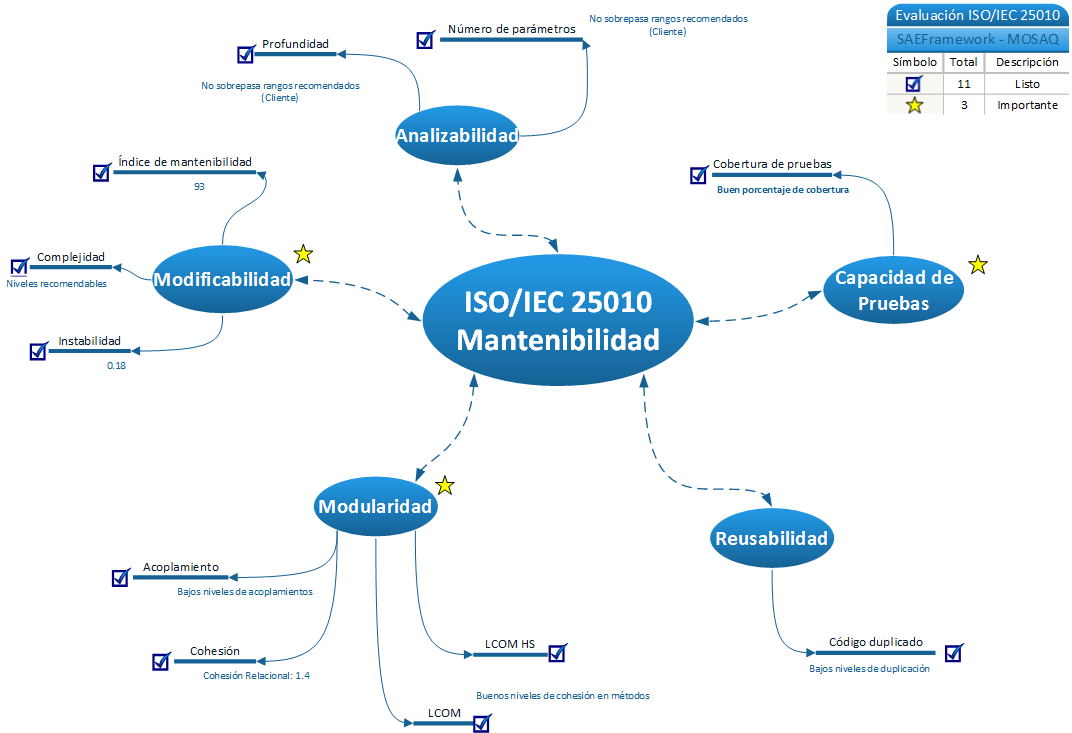
\includegraphics[width=1\textwidth]{img/diagrama.png}
%     \caption{Diagrama resumen de evaluación}
%     \label{fig:diagrama}
% \end{figure}
